\documentclass[12pt,a4paper,ngerman]{article}
\usepackage{listings}
\usepackage{color}

\definecolor{dkgreen}{rgb}{0,0.6,0}
\definecolor{gray}{rgb}{0.5,0.5,0.5}
\definecolor{mauve}{rgb}{0.58,0,0.82}

\lstset{
  language=Python,
  aboveskip=3mm,
  belowskip=3mm,
  showstringspaces=false,
  columns=flexible,
  basicstyle={\small\ttfamily},
  numbers=none,
  numberstyle=\tiny\color{gray},
  keywordstyle=\color{blue},
  commentstyle=\color{dkgreen},
  stringstyle=\color{mauve},
  breaklines=false,
  breakatwhitespace=true,
  tabsize=3
}
\usepackage[ngerman]{babel}
\usepackage[T1]{fontenc}
\usepackage[utf8]{luainputenc}
\usepackage{relsize,etoolbox}
\usepackage[onehalfspacing]{setspace}
\usepackage{hyperref}
\usepackage{rotating}
\usepackage{xcolor}
\usepackage{xparse}
\usepackage[letterspace=900]{microtype}
\usepackage{lmodern}
\usepackage{fancyhdr}
\usepackage{graphicx}
\usepackage{float}
\usepackage{amsmath}
\usepackage{amsfonts}
\usepackage[hang,flushmargin]{footmisc}
\usepackage{tabularx}
\usepackage[font=smaller,labelfont=bf,skip=4pt,figureposition=top]{caption}
\captionsetup[figure]{position=above}
\usepackage{sectsty}
\usepackage{array}
\usepackage{tabu}
\usepackage{verbatim}
\usepackage{enumitem}

\usepackage{helmholtz-ellis-ji-notation}
\usepackage[
  headheight=15pt,
  bmargin=34mm,
]{geometry}
\usepackage[style=numeric]{biblatex}
\usepackage{tablefootnote}

% SET FONT
% \usepackage[cmintegrals,cmbraces]{newtxmath}\usepackage{ebgaramond-maths}\usepackage{helvet}
% \usepackage[cmintegrals,cmbraces]{newtxmath}
% \usepackage[T1]{fontenc}

\usepackage{fontspec}
\usepackage{ebgaramond}
\usepackage{ebgaramond-maths}

% \setmainfont{TeX Gyre Pagella}%% The Palatino from the TeX Gyre Project

% \makesavenoteenv{tabular}
% \makesavenoteenv{table}
\addbibresource{referencesbib.bib}

\sectionfont{\fontsize{14}{15}\selectfont}
\subsectionfont{\fontsize{12}{15}\selectfont}


\setlength\parindent{0pt}
\parskip2mm


% header and footer style
\pagestyle{fancy}
\fancyhead[R]{\slshape}
\fancyhead[L]{\slshape\nouppercase{\rightmark}}
\fancyfoot[C]{\thepage}
\renewcommand{\sectionmark}[1]{\markright{\thesection\ #1}}


% for tables side by side
% https://stackoverflow.com/questions/28678824/in-latex-how-to-put-two-separate-tables-side-by-side-on-top-of-the-paper
\def \hfillx {\hspace*{-\textwidth} \hfill}

% custom commands
\newcommand{\mailto}[1]{\href{mailto:#1}{#1}}

% Titel and author
% \title{
\includegraphics[width=0.8\textwidth]{pictures/folk_logoicemCMYKDT}\\
% Bewegte Stille: \emph{Euler Lattice Spirals Scenery}}
% 
% \author{Levin Eric Zimmermann\\
% {\normalsize \mailto{levin-eric.zimmermann@folkwang-uni.de}}}
% \date{20. September 2020}

\linespread{1.4}
\AtBeginEnvironment{quotation}{\smaller}
\AtBeginEnvironment{quote}{\smaller}

\begin{document}


%************************************TITLE PAGE**************************************%

\begin{titlepage}

\newcommand{\HRule}{\rule{\linewidth}{0.5mm}} % Defines a new command for the horizontal lines, change thickness here

\center% Center everything on the page
 
%----------------------------------------------------------------------------------------
%	HEADING SECTIONS
%----------------------------------------------------------------------------------------

% \textsc{\LARGE Folkwang Universität der Künste}\\[0.5cm] % Name of your university/college
% \textsc{\large Institut für Computermusik und Elektronische Medien}\\[0.5cm] % Minor heading such as course title

\includegraphics[width=0.8\textwidth]{pictures/folk_logoicemCMYKDT}\\[1cm] % Include a department/university logo - this will require the graphicx package
\textsc{\Large Bachelorprojekt Integrative Komposition}\\[0.5cm] % Major heading such as course name
% \textsc{\large Course code}\\[0.5cm] % Minor heading such as course title

%----------------------------------------------------------------------------------------
%	TITLE SECTION
%----------------------------------------------------------------------------------------

\HRule\\[0.4cm]
{\huge mutwo: eine Ereignis zentrierte Umgebung zur Formalisierung zeitbasierter Künste}\\[0.2cm]
\HRule\\[1.5cm]
 
%----------------------------------------------------------------------------------------
%	AUTHOR SECTION
%----------------------------------------------------------------------------------------

\noindent
\begin{minipage}[b]{.25\textwidth}
\end{minipage}%
\begin{minipage}[b]{.25\textwidth}
\begin{flushleft}
\textsc{Autor:}

\textsc{Email:}

\textsc{Matrikelnummer:}

\textsc{Betreuung:}
\end{flushleft}
\end{minipage}%
\begin{minipage}[b]{.5\textwidth}
\begin{flushleft}
Levin Eric Zimmermann % Your name

{\normalsize \mailto{levin-eric.zimmermann@folkwang-uni.de}}

2332991

Prof. Dr. Michael Edwards
\end{flushleft}
\end{minipage}

\vspace{2cm}


%----------------------------------------------------------------------------------------
%	DATE SECTION
%----------------------------------------------------------------------------------------

{\large 01. August 2022}\\[2cm] % Date, change the \today to a set date if you want to be precise

\vfill % Fill the rest of the page with whitespace

\end{titlepage}

% \maketitle
% \thispagestyle{empty}
\newpage


\tableofcontents


\newpage

%%%%%%%%%%%%%%%%%%%%%%%%%%%%%%%%%%%%%%%%%%%%%%%%%%%%%%%%%%%%%%%%%%%%%%%%%%%%%%%%%%%%%%%%%%%%
%%%%%%%%%%%%%%%%%%%%%%%%%%%%%%%%%%%%%%%%%%%%%%%%%%%%%%%%%%%%%%%%%%%%%%%%%%%%%%%%%%%%%%%%%%%%

\section{Einleitung}

%%%%%%%%%%%%%%%%%%%%%%%%%%%%%%%%%%%%%%%%%%%%%%%%%%%%%%%%%%%%%%%%%%%%%%%%%%%%%%%%%%%%%%%%%%%%
%%%%%%%%%%%%%%%%%%%%%%%%%%%%%%%%%%%%%%%%%%%%%%%%%%%%%%%%%%%%%%%%%%%%%%%%%%%%%%%%%%%%%%%%%%%%

\section{Überblick zu Umgebungen computergestützter Komposition}

%%%%%%%%%%%%%%%%%%%%%%%%%%%%%%%%%%%%%%%%%%%%%%%%%%%%%%%%%%%%%%%%%%%%%%%%%%%%%%%%%%%%%%%%%%%%
%%%%%%%%%%%%%%%%%%%%%%%%%%%%%%%%%%%%%%%%%%%%%%%%%%%%%%%%%%%%%%%%%%%%%%%%%%%%%%%%%%%%%%%%%%%%

\section{mutwo}

\subsection{Motivation}

\subsection{Softwarearchitektur}

\subsubsection{Ereignisse}

Ereignisse sind die wichtigsten Elemente in mutwo.
Ein Ereignis ist eine sortierte Sequenz von Vektoren.
Vektoren beschreiben Bewegungen in bestimmten Dimensionen wie zB. Zeit oder räumliche Achsen (X, Y und Z).\footnote{%
        In der Version 0.61.0 von mutwos Kernpaket sind Ereignissen immer nur der Vektor \emph{Dauer} in der Dimension \emph{Zeit} zugeordnet.
        Das ist ein Implementierungsdetail, was in zukünftigen Versionen anders umgesetzt werden mag.
}
Ereignissen sind zusätzlich Parametern zugeordnet, die Eigenschaften der Bewegung definieren.
Parameter könnten für einen Klang zB. eine Tonhöhe sein.
Für eine zweidimensionale räumliche Bewegung wäre potenzieller Parameter eine Farbe, für eine dreidimensionale Bewegung eine bestimmte Gangart.

\begin{figure}[h!]
    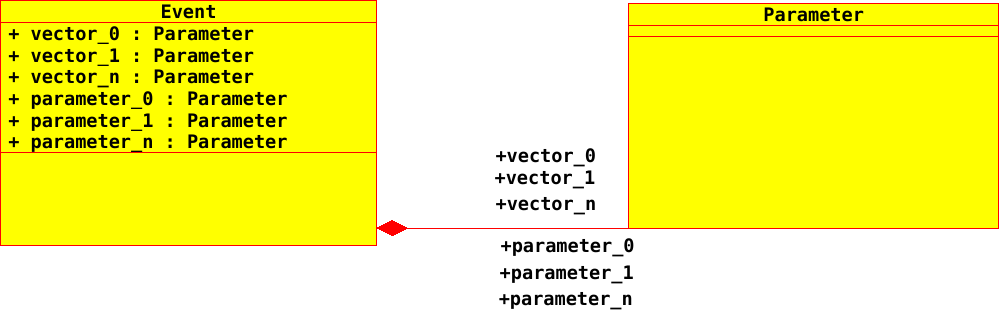
\includegraphics[scale=0.4]{uml_diagrams/event_parameter_basic_150.png}

    \caption{%
        Ein Ereignis kann einen oder mehrere Vektoren enthalten.
        Ein Ereignis kann einen oder mehrere Parameter enthalten.
    }
\end{figure}

In mutwos objektorientiertem Paradigma sind Ereignisse Klassen und deren Instanzen.
Genauso sind Parameter als Klassen umgesetzt.
Zur Vereinfachung gehören Vektoren zum Datentyp Parameter.
Vektoren und Parameter sind Attribute von Ereignissen.

\begin{table}[h!]
    \begin{center}
        \begin{tabular}{l l l l} 
            \hline
            Klassenname & enthält Ereignisse & innere Zeitstruktur & Beispiel \\ [0.5ex] 
            \hline\hline
            \texttt{SimpleEvent} & nein & - & ein Ton, ein Strich \\ 
            \texttt{SequentialEvent} & ja & sequentiell & eine Melodie, ein Quadrat \\ 
            \texttt{SimultaneousEvent} & ja & simultan & polyphoner Satz, zwei Rechtecke \\ [1ex] 
            \hline
        \end{tabular}
    \end{center}

    \caption{Kernereignisse in mutwo}
\end{table}

Ereignisse können andere Ereignisse enthalten oder keine anderen Ereignisse enthalten.
Falls Ereignisse andere Ereignisse enthalten, können die enthaltenen Ereignisse wiederrum iterativ weitere Ereignisse enthalten (Verschachtlung).
Falls ein Ereignis Ereignisse enthält, können diese entweder simultan oder sequenziell angeordnet sein.
Mit den drei Ereignisklassen \texttt{SimpleEvent}, \texttt{SequentialEvent} und \texttt{SimultaneousEvent} sind alle Möglichkeiten darstellbar.

\begin{figure}[h!]
    \begin{center}
        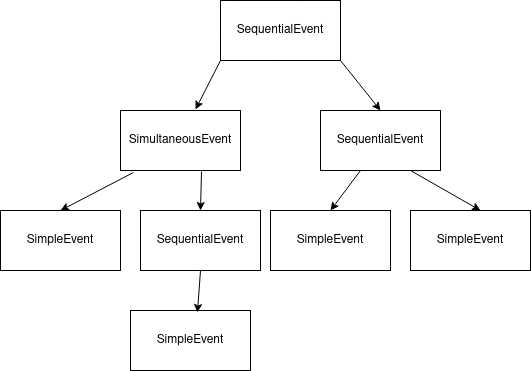
\includegraphics[scale=0.5]{pictures/nested_event.png}

        \caption{Exemplarische Verschachtlung von Ereignissen}
    \end{center}
\end{figure}


\subsubsection{Parameter}

Parameter repräsentieren generische Kategorien, die Ereignissen zugeordnet werden.
Generische Kategorien können beispielweise eine Farbe, eine Tonhöhe oder ein Luftdruck sein.

In mutwos Design sind Parameter als abstrakte Klassen definiert, die eine minimale, öffentliche Programmierschnittstelle beschreiben.
Diese minimale Schnittstelle versucht Parameter auf eine kompakte Identität zu reduzieren, die unabhängig ist von bestimmten Traditionen.
Wenn möglich besteht diese kompakte Identität aus nur einem Wert (zB. Zeichenkette oder Zahl).
Wenn möglich ist der Wert implizit einer physikalischen Einheit zugeordnet.

\begin{table}[h!]
    \begin{center}
        \begin{tabular}{l l l l} 
            \hline
            Parameter & Klassenname & Elementares Klassenattribut & Einheit \\ [0.5ex] 
            \hline\hline
            Tonhöhe & \texttt{Pitch} & \texttt{frequency} & Hertz \\ 
            Tonhöhenintervall & \texttt{PitchInterval} & \texttt{interval} & Cents \\ 
            Dauer & \texttt{Duration} & \texttt{duration} & beats \\ 
            Text & \texttt{Lyric} & \texttt{phonetic\_script} & X-SAMPA\footnote{%
                Das ``Extended Speech Assessment Methods Phonetic Alphabet' ist eine Möglichkeit die phonetischen IPA Symbole in ASCII darzustellen.~\cite{xsampaWikipedia}
            } \\ 
            Lautstärke & \texttt{Volume} & \texttt{amplitude} & Volt \\ [1ex] 
            \hline
        \end{tabular}
    \end{center}

    \caption{Liste exemplarischer Ein-Wert-Parameter}
\end{table}

Andere Bestandteile mutwos erwarten nur die minimal--definierte Schnittstelle.
Das ermöglicht Benutzern die Implementierung einer Repräsentation einer Kategorie, die der jeweiligen Denkweise entspricht.
Das Design mutwos versichert, dass die von Benutzern hinzugefügten Repräsentationen mit anderen Bibliothekskomponenten kompatibel sind.

\begin{figure}[h!]
    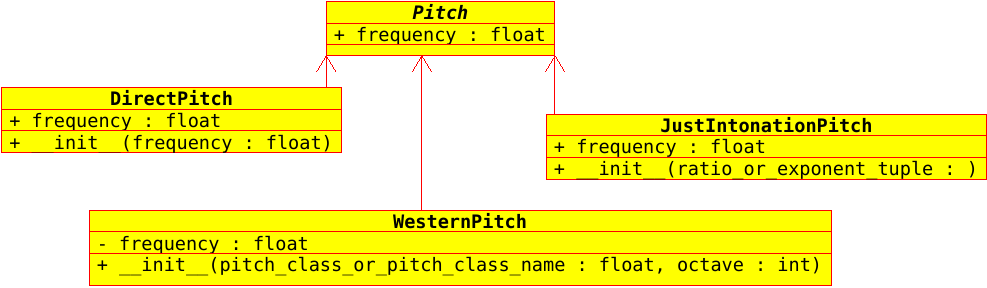
\includegraphics[scale=0.4]{uml_diagrams/pitches.png}

    \caption{%
        Schematische Darstellung eines Parameter und unterschiedlicher Subklassen.
        Die Subklassen werden mit unterschiedlichen Argumenten initialisiert.
    }

\end{figure}

\subsubsection{Übersetzer}

Ein Übersetzer transformiert eine Entität.
Entitäten sind entweder Objekte in Python oder externe Dateien.\footnote{%
    Objekte in Python können Instanzen von mutwo internen Klassen, dritten Bibliotheken oder nativen Klassen sein.
    Externe Dateien umfassen beispielweise Mididateien oder Textdateien.
}
Transformieren bedeutet hier entweder eine Veränderung des Inhalts oder eine Veränderung des Formats.


\begin{table}[h!]
    \hspace{-0.5cm}
        \smaller
        \begin{tabular}{l l l l} 
            \hline
            Klassenname & Eingangsentität & Ausgangsentität & Typ \\ [0.5ex] 
            \hline\hline
            \texttt{EventToMidiFile} & Instanz einer Ereignisklasse & Standard Midi File (SMF) & Format \\ 
            \texttt{MidiFileToEvent} & Standard Midi File (SMF) & Instanz einer Ereignisklasse & Format \\ 
            \texttt{TwoPitchesToCommonHarmonicTuple} & Zwei Tonhöheninstanzen & Instanzen gemeinsamer Harmonischer & Inhalt \\ 
            \texttt{PitchToTabulaturaPitch} & Tonhöheninstanz & Tonhöheninstanz & Inhalt \\ [1ex] 
            \hline
        \end{tabular}

    \caption{Exemplarische Übersetzer}
\end{table}


Übersetzer in mutwo folgen bedingt einem funktionalem Paradigma, dh.\ ein Übersetzer verändert nicht die Eingangsentität, sondern erzeugt eine neue, unabhängige Entität.
Das vereinfacht das Übersetzen derselben Entität mit unterschiedlichen Übersetzer.

\subsubsection{Generatoren}

Generatoren liefern zumeist generische Daten, die für generative Kunst nützlich sein mögen.
Generatoren umfassen Funktionen, Klassen, Konstanten oder andere Objekte.
Die Rückgabewerte der Funktionen und Klassen sind häufig Python native Objekte, die von Benutzern kreativ angewendet werden können.

\begin{table}[h!]
    \begin{center}
        \begin{tabular}{l l} 
            \hline
            Objekt & Beschreibung \\ [0.5ex] 
            \hline\hline
            \texttt{reflected\_binary\_code} & Erzeugt variable Gray-Codes \\
            \texttt{TUNEABLE\_INTERVAL\_TUPLE} & intonierbare Intervalle nach Marc Sabat \\
            \texttt{ActivityLevel} & Zyklen der Werte 0 und 1 nach Michael Edwards \\ [1ex] 
            \hline
        \end{tabular}
    \end{center}

    \caption{Exemplarische Generatoren}
\end{table}

\subsubsection{Module und Packete}

Der Quellcode von mutwo ist nach rigiden Regeln strukturiert.
Die Struktur basiert auf Pythons System von verschachtelten Modulen, Importe und Paketen.
Grundsätzliche Absicht der rigiden Struktur ist eine einfache Verwendung für Benutzer und eine Vereinfachung der Entwicklung und Instandhaltung eines komplexen Softwareprojekts.

Der Paketname der Bibliothek ist mutwo.
Pakete können im Python-Ökosystem auf der Plattform \emph{pypi} verwaltet werden.
Mit dem standardisierten Pythonpaketmanager \emph{pip} können Pakete von \emph{pypi} installiert werden.

\lstset{language=bash}

\begin{lstlisting}
    pip3 install mutwo
\end{lstlisting}

Das Paket mutwo ist in unterschiedliche Module geteilt.
Die unterschiedlichen Module korrelieren mit den zuvor beschriebenen elementaren Bestandteile von mutwo.
Sie werden flankiert von zusätzlichen Hilfsmodulen.

\begin{table}[h!]
    \begin{center}
        \begin{tabular}{l l} 
            \hline
            Modulname & Modulbeschreibung \\ [0.5ex] 
            \hline\hline
            \texttt{configurations} & Globale modulübergreifende Konfigurationsvariablen \\
            \texttt{constants} & Globale modulübergreifende Konstanten \\
            \texttt{converters} & Importieren und Exportieren von Daten, Übersetzen interner Strukturen \\
            \texttt{events} & Definition verschiedener Ereignisklassen \\
            \texttt{generators} & Generierung von für künstlerische Arbeiten hilfreiche Daten \\
            \texttt{parameters} & Klassen, deren Instanzen Ereignisattributen zugeordnet werden \\
            \texttt{version} & Versionsdefinition des Moduls \\
            \texttt{utilities} & Hilfsmethoden, Errordefinition \\ [1ex] 
            \hline
        \end{tabular}
    \end{center}

    \caption{Moduldefinitionen}
\end{table}

Module oder Pakete können in Python auf unterschiedliche Weisen importiert werden.
Die folgende Zeile dokumentiert die in mutwo bevorzugte Weise:

\lstset{language=Python}

\begin{lstlisting}
    from mutwo import parameters
\end{lstlisting}

Mutwo Module enthalten direkt die verwendbaren Objekte.
Sie können nur eine limitierte Anzahl bestimmter Submodule enthalten.
Weil die Regel für alle mutwo Module gilt ist sie einfach zu verstehen für neue Benutzer.
Sie korreliert mit der fünften Zeile des \emph{Zen of Python}:

\begin{quote}
    ``Flat is better than nested.''
\end{quote}

Folgende Tabelle beschreibt die möglichen Submodule eines Moduls.

\begin{table}[h!]
    \begin{center}
        \begin{tabular}{l l} 
            \hline
            Modulsuffix & Modulbeschreibung \\ [0.5ex] 
            \hline\hline
            \texttt{abc} & Abstrakte Klassen, Definition der gemeinsamen API \\
            \texttt{configurations} & Globale modifizierbare Variablen zur Modulkonfiguration \\
            \texttt{constants} & Globale Konstanten des Moduls \\
            \hline
        \end{tabular}
    \end{center}

    \caption{Submoduldefinitionen}
\end{table}


\begin{table}[h!]
    \begin{center}
        \begin{tabular}{l l l} 
            \hline
            Packetname & Modulprefix & Packetbeschreibung \\ [0.5ex] 
            \hline\hline
            \textbf{mutwo.core} & \texttt{core} & Kunstform-, medien- und kulturagnostische Objekte \\
            \textbf{mutwo.music} & \texttt{music} & Musikspezifische Objekte \\
            \textbf{mutwo.midi} & \texttt{midi} & Importieren und Exportieren von SMF\footnote{Standard Midi Files} \\
            \hline
        \end{tabular}
    \end{center}

    \caption{Exemplarische Auswahl verschiedener mutwo Pakete}

\end{table}


\subsection{Eigenschaften und Limitierungen}

\subsection{Beispiel-orientierte Einführung}

%%%%%%%%%%%%%%%%%%%%%%%%%%%%%%%%%%%%%%%%%%%%%%%%%%%%%%%%%%%%%%%%%%%%%%%%%%%%%%%%%%%%%%%%%%%%
%%%%%%%%%%%%%%%%%%%%%%%%%%%%%%%%%%%%%%%%%%%%%%%%%%%%%%%%%%%%%%%%%%%%%%%%%%%%%%%%%%%%%%%%%%%%

\subsection{Fallstudien}

\subsubsection{thanatos trees for Tim Pauli}

\subsubsection{ohne Titel (2) und ohne Titel (3)}

\section{Zusammenfassung}

\subsection{Richtungen weiterer Entwicklungen}

\subsection{Evaluation}

\newpage

\appendix

\printbibliography

\newpage

\listoffigures

\newpage


\end{document}
